\chapter{Coletando Feedback}
\label{chap:coletando}

Neste capítulo, vamos entender como tanto o feedback explícito, quanto implícito, são coletados no nosso sistema.

\section{Feedback Explícito}

No nosso sistema, coletamos duas métricas de feedback explícito: o tempo de perfil e a ação de exploração.

\begin{figure}[t]
	\centering
	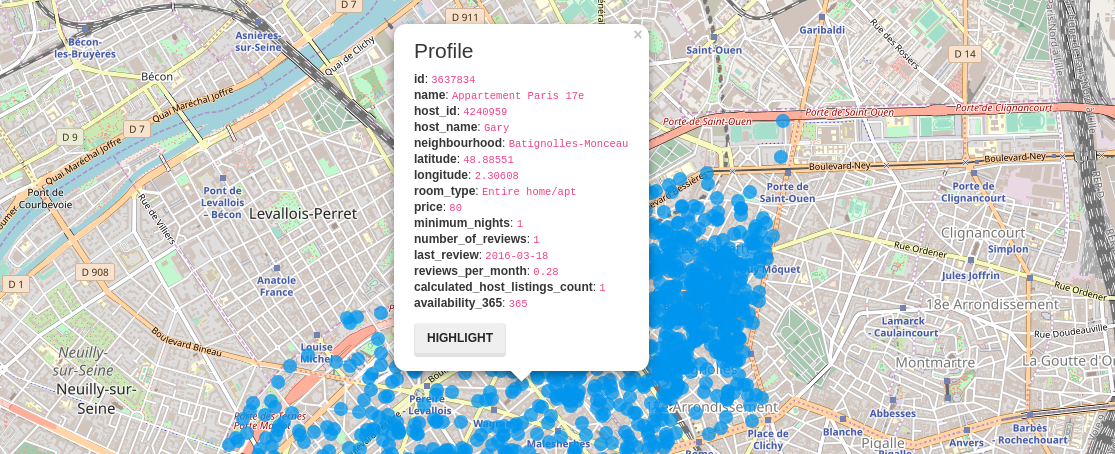
\includegraphics[width=\columnwidth]{imagens/perfil-do-ponto}
	\caption{GeoGuide: Perfil do Ponto}
	\label{fig:perfil-do-ponto}
	\vspace{-10pt}
\end{figure}

\subsection{Tempo de Perfil}

O tempo de perfil refere-se ao tempo que o usuário se dedica a analisar o perfil de um determinado ponto no conjunto de dados, como na Figura \ref{fig:perfil-do-ponto}. Por exemplo, em um conjunto de dados sobre avaliações de restaurantes, um usuário tende a passar mais tempo analisando o perfil de um restaurante que ele tenha interesse.

Quanto mais longo um usuário passa ativamente analisando um perfil, mais interesse o analista está demostrando explicitamente para nosso sistema. Dessa forma, os pontos com tempo de perfil maiores são levados como referência durante a exploração.

\subsection{Exploração}

A exploração refere-se ao ato do usuário decidir explorar um determinado ponto. Esse ato é coletado através do botão ``Explore'' abaixo do perfil do ponto como mostra a Figura \ref{fig:perfil-do-ponto}.

Ao explorar um determinado ponto, o analista está explicitamente indicando que esse ponto é relevante ao seu interesse e gostaria de sugestões baseadas nesse ponto. Nosso sistema, através desse feedback explícito, da coleta de feedback implícido e nos índices de relevância e diversidade, destaca ao usuário $k$ pontos relevantes. Esse processo de destacamento será discutido no Capítulo \ref{chap:guiando}.

\section{Feedback Implícito}

Para coleta do feedback implícito, utilizamos os movimentos do mouse do analista para entender para onde e em quê seu interesse está voltada \cite{arapakis2014understanding}. Como podemos ver na Figura \ref{fig:interface}, a interface do nosso sistema é uma mapa em tela cheia. Quando o usuário está explorando o mapa, nosso sistema está coletando os pontos geográficos por onde o mouse se movimenta.

Cada ponto geográfico $p$ coletado através do rastreio dos movimentos do mouse possue os seguintes atributos: latitude, longitude e data. Dessa forma, cada ponto $p$ é definido no contexto espacial e temporal.

O processo de captura é agrupado em iterações. Cada iteração dura $t$ segundos e no final de cada iteração, os pontos são clusterizados utilizando o algoritmo ST-DBScan. Em seguida, os clusters são utilizados para encontrar as regiões mais exploradas pelo analista através do algoritmo Quickhull.

Esse processo de rastrear os pontos $p$, clusterizar e encontrar as regiões é realizado a cada iteração. Em $T$ segundos, as regiões encontradas nas iterações anteriores são agrupadas e sobrepostas. Uma vez sobrepostas, se houver interseções, essas interseções são definidas como regiões densas interessantes.

% Poligonos...

% ST-DBScan

% Quickhull

% Interseção

% Perfil

% Numericos: Pandas
% Texto: Counter
% Categóricos: Counter
% Datetime: timeseries

\begin{figure}[t]
	\centering
	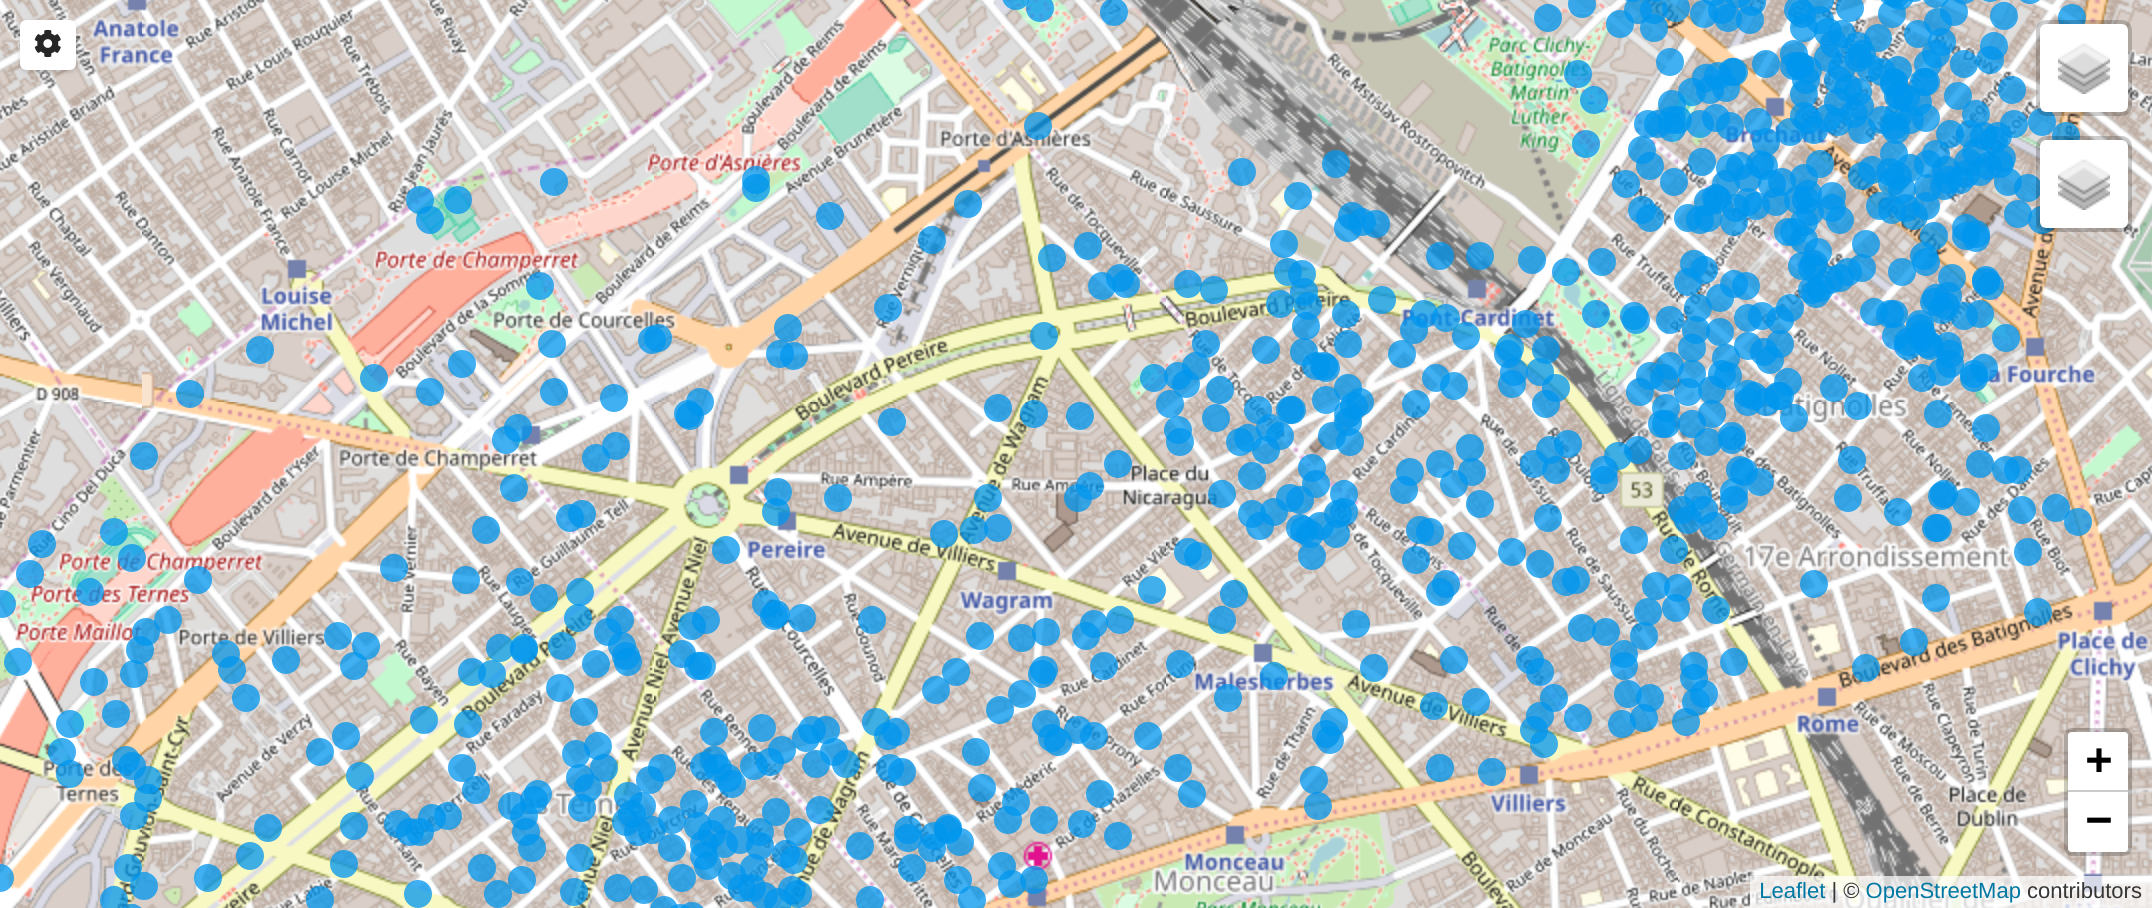
\includegraphics[width=\columnwidth]{imagens/interface}
	\caption{GeoGuide: Inteface}
	\label{fig:interface}
	\vspace{-10pt}
\end{figure}